\documentclass[5p,twocolumn]{elsarticle}
\usepackage{graphicx}
\usepackage{booktabs}
\biboptions{numbers,sort&compress}
\usepackage[colorlinks=true,linkcolor=blue,citecolor=blue,urlcolor=blue]{hyperref}
\pdfstringdefDisableCommands{%
  \def\corref#1{}%
  \def\cnotenum#1{}%
}
\usepackage{amsmath}
\usepackage{caption}
\usepackage{dblfloatfix}
\usepackage{cuted}
\setlength{\parindent}{1em}
\setlength{\parskip}{0pt}
\setlength{\textfloatsep}{8pt plus 2pt minus 2pt}
\setlength{\floatsep}{7pt plus 2pt minus 2pt}
\setlength{\intextsep}{7pt plus 2pt minus 2pt}
\setlength{\dbltextfloatsep}{8pt plus 2pt minus 2pt}
\setlength{\dblfloatsep}{7pt plus 2pt minus 2pt}
\captionsetup{font=footnotesize,labelfont=bf,skip=3pt}
\emergencystretch=3em

\journal{Journal of Nuclear Materials}

\begin{document}
\begin{frontmatter}
\title{\texorpdfstring{Acceptance-gated bonded-template DEM reveals localized fracture sequences in Li$_4$SiO$_4$ ceramic breeder beds}{Acceptance-gated bonded-template DEM reveals localized fracture sequences in Li4SiO4 ceramic breeder beds}}
\author[aff1,aff2]{Jian Wang\corref{cor1}}
\ead{wjfttt@mail.ustc.edu.cn}
\author[aff1]{Siyu Wang}
\author[aff1]{Hang Zhang}
\author[aff2]{Ming-Zhun Lei}
\author[aff1,aff2]{Wei Wen}
\author[aff2]{Qi-Gang Wu}
\author[aff1]{Gang Shen}
\author[aff1]{Haishun Deng}
\cortext[cor1]{Corresponding author.}
\address[aff1]{Anhui University of Science and Technology, Huainan, Anhui 232001, China}
\address[aff2]{Institute of Plasma Physics, Chinese Academy of Sciences, Hefei, Anhui 230031, China}











\begin{abstract}

Lithium orthosilicate pebbles are functional ceramic breeder materials whose mechanical degradation can alter bed stiffness, contact topology and purge-gas pathways in solid breeder blankets. Existing single-pebble and bed-compression studies provide crush-load and bulk-response information, but they do not resolve the hidden time order of mother-pebble fracture inside an opaque random bed. Here we develop a bonded-template discrete-element workflow in which each nominal 1.0 mm Li$_4$SiO$_4$ mother pebble is represented by 500 bonded subparticles, inserted intact into a gravity-settled bed and allowed to break only during subsequent compression. A weak-plane template reproduces the target crush-load scale and split-type morphology as a current calibration candidate; resolution and loading-rate checks preserve first-break displacement and fragment topology while bounding peak-load sensitivity. The corrected 100-mother-pebble bed route passes zero-pre-damage, native force graph connectivity and gravity-baseline-corrected force-balance gates before fracture is interpreted. Three corrected 60 micrometre bed compressions show distinct event paths: a pilot loses five of 493,500 internal bonds in one upper-bed mother pebble, a second random bed remains intact even under 0.5x and 0.25x strength audits, and a third random bed develops delayed microcracking after 50 micrometres with ten final broken bonds in two upper-bed mother pebbles. The output is a set of material-degradation state variables: event time, damaged mother-pebble identity, bond-loss increment, native force graph connectivity and macroscopic force relaxation. The workflow converts crushable breeder-bed simulations into auditable fracture-event sequences for nuclear-materials assessment, while larger ensembles remain required before predictive lifetime or design-margin statements are made.


\end{abstract}

\begin{keyword}
lithium orthosilicate; ceramic breeder material; pebble bed; bonded-particle DEM; pebble crushing; fracture-event sequence; nuclear materials
\end{keyword}
\end{frontmatter}

\section{Introduction}

Lithium orthosilicate ceramic pebbles are candidate tritium-breeder materials for helium-cooled solid breeder blankets \cite{Piazza2002CeramicBreederMaterials,Reimann2000ThermomechanicalPebbleBeds}. In this nuclear-materials application, the breeder bed is both a functional ceramic inventory and a mechanically loaded granular assembly: it provides lithium for tritium generation, conducts heat toward coolant structures, and must retain connected purge-gas pathways for tritium extraction. Pebble crushing can change contact networks, local bed stiffness, thermal pathways and helium purge-flow resistance, thereby affecting the interpretation of ceramic breeder-bed integrity and service degradation. Recent cyclic-compression experiments on Li$_4$SiO$_4$ beds further show that increasing stress and temperature increase particle breakage and the fraction of small fragments, while independently prepared crushed beds exhibit increasing helium pressure drop with breakage ratio \cite{CrushedPebblePressureDrop2024,Fang2026Li4SiO4BedCrushing}.


Single-pebble crush tests provide essential contact-strength, size-effect, failure-initiation and elastic-response targets, and bed-compression experiments reveal collective stiffness, compaction and failure trends \cite{PlateMaterialLi4SiO4,Zhao2013FailureInitiationLi4SiO4,Annabattula2014SizeDependentCrush,Bhartia2020ElasticResponse,PreliminaryLi4SiO4StructuralPerformance,ZaccariLoFrano2009CeramicPebbleBeds}. However, experiments on opaque beds cannot easily identify which mother pebble breaks first, whether damage remains local or spreads laterally, or how fracture events evolve under increasing compression. Existing DEM studies have advanced breeder-bed analysis by relating macroscopic response to coordination number, contact-force distributions and packing structure, and by estimating crush probability from single-pebble strength distributions \cite{An2007DEMCeramicBreederBeds,GanKamlah2010DEMPebbleBeds,CrushProbabilityPebbleBed2011,Wang2021CrushableCeramicPebbleBed}. The unresolved gap is event-level: most bed-scale models still treat pebbles as rigid particles, or infer failure after the fact, so they cannot directly produce a time-ordered, mother-pebble-resolved fracture sequence.


Bonded-particle DEM provides a route to this missing representation because a brittle object can be assembled from subparticles connected by breakable bonds, allowing bond loss and fragment generation to be followed directly \cite{PotyondyCundall2004}. Recent Li$_4$SiO$_4$ sub-ball DEM work has shown that such models can reproduce size-dependent single-pebble crush behaviour \cite{Li4SiO4SizeDEM2023}, and prior breeder-bed simulations have explored crushable-bed response \cite{Wang2021CrushableCeramicPebbleBed,CrushableDEMPebbleBed2026}. For blanket design, however, a method must also ensure that a breakable pebble is inserted into a random bed without artificial pre-damage; otherwise the simulated fracture sequence may partly reflect initialization artefacts rather than service loading. This zero-precompression-damage requirement becomes especially important when the results are used to reason about safety margins, lifetime degradation and transport-path preservation.


We therefore introduce a locked-template workflow for fracture-resolved breeder-bed compression, schematized in Fig. 1. Whole-pebble proxy spheres first settle under gravity to create a random packing. The settled centres are then replaced by 500-subparticle bonded templates, which are created far apart to form only internal bonds and translated as intact groups into the packed bed. This separates bed generation from pebble crushing, verifies zero internal bond loss before loading, and enables mother-pebble-resolved fracture events to be extracted by comparing internal bond graphs across compression dumps. The resulting event database is intended as mesoscopic evidence for how local pebble damage may initiate and propagate in solid breeder blankets, rather than as a final design rule. In this framing, bond-loss increments, damaged-pebble identity, native reachability and force relaxation are treated as computed state variables for ceramic breeder-material degradation.


\begin{figure*}[!t]
\centering
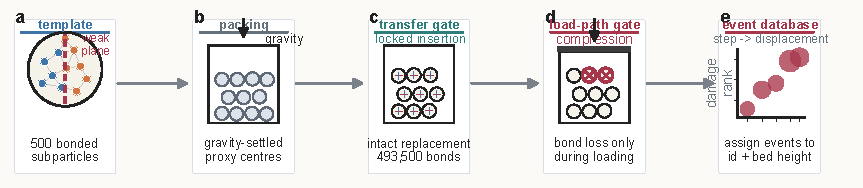
\includegraphics[width=0.92\textwidth]{fig1_workflow.pdf}
\caption{Locked-template workflow for fracture-resolved Li$_4$SiO$_4$ breeder-bed compression. A nominal 1 mm mother pebble is represented by a 500-subparticle bonded template. Proxy spheres first settle under gravity without internal bonds. The settled proxy centres are then replaced by intact bonded templates, so internal bond failure is absent during bed formation and is activated only during compression. The corrected route adds explicit acceptance gates: zero internal-bond loss before loading, native mother-mother force connectivity, six-wall force output and gravity-baseline-corrected incremental force balance. Bond-state records are then converted into a mother-pebble-resolved fracture-event database. The workflow combines bonded-particle fracture modelling with ceramic breeder-bed DEM concepts \cite{PotyondyCundall2004,An2007DEMCeramicBreederBeds,GanKamlah2010DEMPebbleBeds}.}
\label{fig:workflow}
\end{figure*}


\section{Results}

\subsection{A bonded 1 mm template provides an internal failure state for each pebble}

We first generated a nominal 1.0 mm Li$_4$SiO$_4$ pebble from 500 spherical subparticles. The final non-overlapping template produced a stable internal bond network and no preloading failure. A homogeneous strength scan showed the intended trend: increasing bond strength increased peak compressive load while reducing final bond loss. However, homogeneous load-matched templates failed mainly by surface chipping, leaving one large fragment and several single-subparticle chips.


To obtain a more realistic split-type failure mode, we introduced a weak-plane template in which cross-plane bonds were assigned lower strength and a shorter bond-creation distance. The calibration evidence is summarized in Fig. 2. The selected x-normal weak-plane template reached a peak top force of 18.64 N and a peak bottom force of 18.07 N, while the final intact-bond graph contained two major fragments of 227 and 224 subparticles plus small chips. The corresponding three-dimensional fragment morphology is provided as Supplementary Fig. S1. Pilot orientation and strength-multiplier scans retained the two-major-fragment mode while producing peak-load scatter, supporting the use of template orientation and sample strength as stochastic variables in later ensemble studies.


\begin{figure*}[!t]
\centering
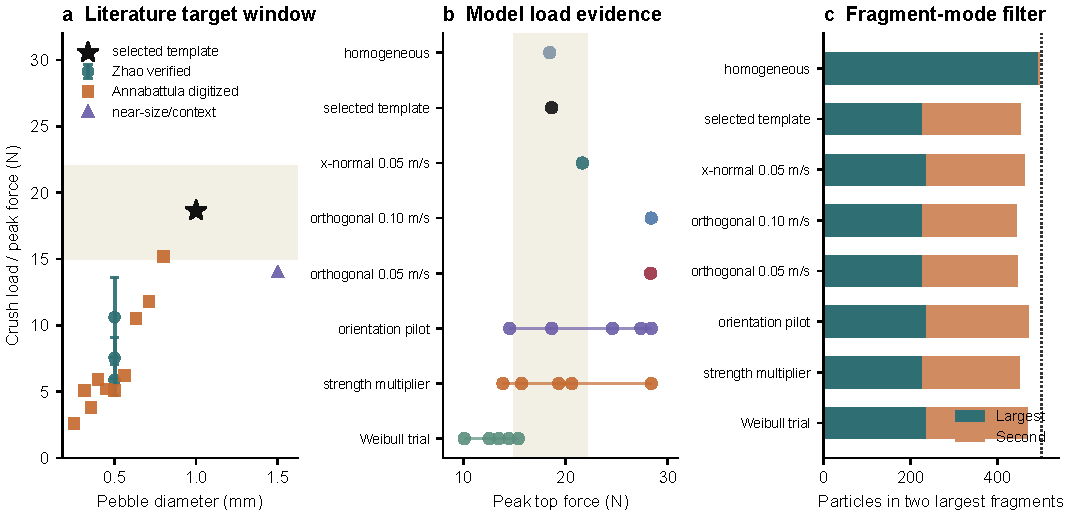
\includegraphics[width=0.92\textwidth]{single_pebble_calibration_evidence.pdf}
\caption{Single-pebble calibration evidence for the current 500-subparticle template. In panels b and c, "homogeneous" denotes a uniform-bond-strength template, "selected template" denotes the x-normal weak-plane calibration candidate, "orthogonal" denotes weak-plane orientation variants, "strength multiplier" denotes deterministic bond-strength scaling, and "Weibull trial" denotes a stochastic strength sample. The selected weak-plane template lies in the provisional 1 mm crush-load target window and preserves a two-major-fragment mode, but it is treated as a current calibration candidate rather than a final Li$_4$SiO$_4$ material law. The load window and interpretation are anchored to published Li$_4$SiO$_4$ crush and elastic-response studies \cite{PlateMaterialLi4SiO4,Annabattula2014SizeDependentCrush,Bhartia2020ElasticResponse,Li4SiO4SizeDEM2023}.}
\label{fig:single-pebble-calibration}
\end{figure*}


\subsection{Resolution and loading-rate checks bound the remaining numerical sensitivity}

We next repeated the single-pebble calculation with controlled 250-, 500- and 1000-subparticle templates using the same random seed, weak-plane law and dimensionless bond-creation cutoffs (Fig. 3). First-break displacement remained within 0.0950-0.0965 mm across all three resolutions. The final two largest fragments contained 117 and 103 subparticles for the 250-subparticle template, 237 and 230 for the 500-subparticle template, and 446 and 445 for the 1000-subparticle template. Thus, first-break onset and split topology are robust over the tested resolution range. Peak top force increased from 17.91 N at 250 subparticles to 19.40 N at 500 and 22.64 N at 1000, showing moderate residual load-scale sensitivity rather than strict convergence.


A separate matched-boundary rate set used the same 500-subparticle template, plate gap and timestep at 0.10, 0.05 and 0.03 m s$^{-1}$. Peak top forces were 19.40, 18.84 and 17.35 N, respectively, while first-break displacement remained within 0.0945-0.0950 mm. All three rates retained two dominant fragments containing approximately 45-47\% of the subparticles each. The 0.03 m s$^{-1}$ run therefore lowers the peak load by 10.5\% relative to 0.10 m s$^{-1}$ but preserves the onset window and final split mode. These checks support the use of the 500-subparticle template for event-sequence screening while retaining a conservative uncertainty bound on absolute peak load.


\begin{figure*}[!t]
\centering
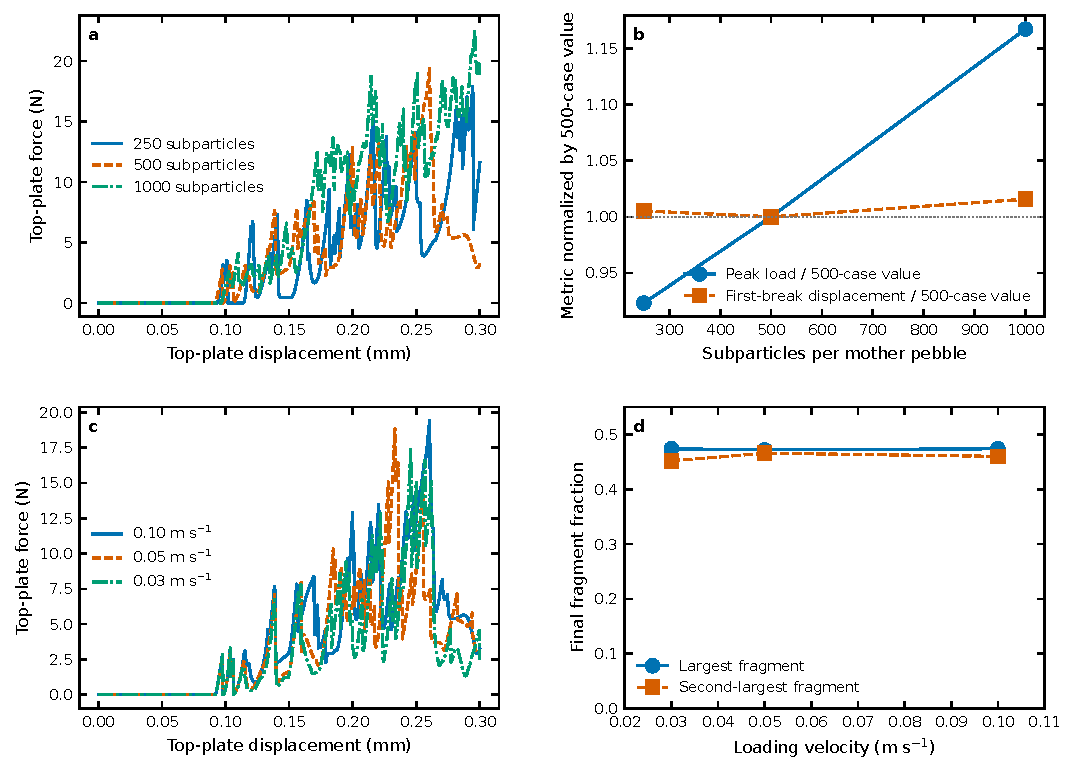
\includegraphics[width=0.92\textwidth]{jnm_single_pebble_validation.pdf}
\caption{Subparticle-resolution and loading-rate sensitivity of the single-pebble template. a, Force-displacement curves for 250, 500 and 1000 subparticles. b, Peak load and first-break displacement normalized by the 500-subparticle result. c, Matched-boundary force-displacement curves at 0.10, 0.05 and 0.03 m s$^{-1}$. d, Final largest- and second-largest-fragment fractions across loading rates. Onset and split topology are robust, whereas peak load retains moderate resolution and rate sensitivity. The checks follow the established need to assess sub-ball discretization and loading protocol in brittle-pebble DEM calibration \cite{PotyondyCundall2004,Li4SiO4SizeDEM2023}.}
\label{fig:single-pebble-validation}
\end{figure*}


\subsection{Surface-supported template transfer creates a connected corrected bed}

The first locked-template bed calculations showed why insertion validation must be treated as part of the material model rather than as a numerical convenience. A random 500-subparticle template can be intact as a single pebble but still have insufficient directional support near some surface directions after proxy-to-template replacement. We therefore introduced a surface-supported template for bed insertion. The selected surface-supported geometry improved the q05, median and q95 directional diameter metrics to 0.99355, 0.99639 and 0.99889 mm, respectively, while retaining a split-type single-pebble failure mode with two dominant fragments of 220 and 213 subparticles after compression.


The corrected bed was then generated by rigid-clump gravity settling followed by bonded-template transfer. The 100-mother-pebble pilot contains 50,000 subparticles after transfer. The initial internal-bond count is exactly 493,500, corresponding to 100 templates with 4,935 internal bonds each, and the transferred bonded coordinates reproduce the rigid-clump positions at nanometre-scale precision. Native contact diagnostics after rigid settling identify 164 inter-pebble candidate edges, a largest connected component containing 99 of 100 mother pebbles and 27 bottom-contacting pebbles. This corrected initialization replaces an earlier diagnostic route, retained only in the audit record, which showed that zero pre-damage alone is insufficient without a verified load path.


\subsection{Pre-damage force-transmission gates prevent false fracture interpretation}

Before any fracture sequence was interpreted, the corrected bed was compressed by five 1 micrometre step-relaxation increments. The acceptance gate required four simultaneous conditions: zero internal-bond loss, native mother-mother contact-force connectivity, six-wall force output and gravity-baseline-corrected incremental force balance. The gravity baseline is necessary because the bottom wall already carries bed self-weight before top compression.


The low-stiffness step-relaxed validation case passed the pre-damage gate at 5 micrometres of top-wall displacement. The top-wall load was 1.713e-4 N and the gravity-baseline-corrected six-wall incremental force was 1.704e-4 N, giving a residual of 0.542\%. The intact-bond count remained 493,500 throughout the run. Native local-contact output at the final state contained 165 mother-mother force edges and 298 inter-pebble subcontacts; the top-loaded set reached 99 of 100 mother pebbles and 26 bottom-contacting pebbles.


Restoring the contact modulus toward the single-pebble value required a second gate. Direct restoration to 9.0e10 Pa caused 14 internal bonds to fail without top-wall compression, so it was excluded from fracture interpretation. A short modulus screen retained zero pre-damage at 5.0e8, 5.0e9 and 2.0e10 Pa, but produced spurious bond loss at 3.0e10 and 5.0e10 Pa. The current fracture entry protocol uses a restored contact modulus of 1.5e10 Pa with 10,000 pre-compression relaxation steps and five 1 micrometre step-relaxation increments; this value is a gate-passing numerical protocol, not as a measured material stiffness. At 5 micrometres, this entry protocol retained all 493,500 internal bonds, gave a final top-wall load of 1.638e-2 N and a gravity-baseline-corrected six-wall incremental force of 1.559e-2 N, corresponding to a 4.799\% balance residual. The native force graph remained spanning, with 36 mother-mother edges and top-loaded reachability to 28 mother pebbles, including three bottom-contacting pebbles.


\begin{figure*}[!t]
\centering
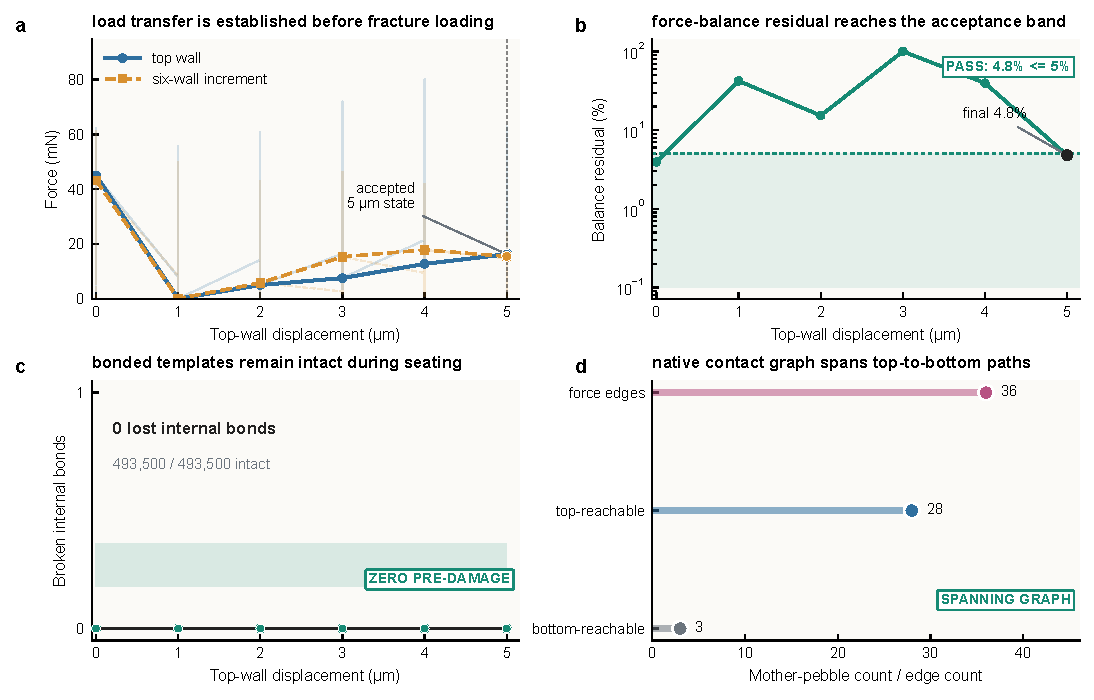
\includegraphics[width=0.92\textwidth]{pb007_acceptance_gate_validation.pdf}
\caption{Corrected pre-damage force-transmission validation. The corrected route validates the 100-mother-pebble bed before fracture interpretation. a, Relaxed endpoint top-wall force and gravity-baseline-corrected six-wall incremental force during the accepted 5 micrometre entry protocol; faint traces show within-step relaxation. b, Incremental force-balance residual at relaxed endpoints, with the final value entering the 5\% gate. c, Internal-bond damage remains zero throughout the entry protocol. d, Native final-state force-network gate, showing 36 mother-mother force edges, 28 top-reachable mother pebbles, three bottom-contacting pebbles reachable from the top-loaded set and a spanning graph. This acceptance-gated workflow follows the need to separate contact-network formation from brittle-particle failure in crushable breeder-bed simulations \cite{PotyondyCundall2004,Wang2021CrushableCeramicPebbleBed,CrushableDEMPebbleBed2026}.}
\label{fig:pb007-force-validation}
\end{figure*}


\subsection{Corrected compression localizes the first fracture sequence in one upper pebble}

The corrected 60 micrometre compression pilot was launched from the 1.5e10 Pa gate-passing entry protocol with periodic local internal-bond dumps and native pair/wall contact dumps. At the final displacement, 493,495 of 493,500 internal bonds remained intact. The five lost bonds were not distributed through the bed; all localized in mother pebble 78, which lies near the top of the bed with \texttt{pebble\_z\_mm=2.96658} and rank from top 2. The mother-pebble event table records three increments: two lost internal bonds at 25 micrometres, two additional lost bonds at 35 micrometres and one additional lost bond at 60 micrometres. No other mother pebble shows internal-bond loss in this pilot.


The native force-network snapshots show that damage was embedded in an already spanning load-bearing graph. Inter-mother force edges increased from 55 at 10 micrometres to 67 at 25 micrometres and 79 at 40 micrometres, while the number of mother pebbles reachable from the top-loaded set increased from 48 to 58 and then 65. By 55 micrometres, the graph remained spanning but reorganized to 67 inter-mother edges and 56 top-reachable mother pebbles. The final native graph contained 74 inter-mother edges, 119 inter-pebble subcontacts, 57 mother pebbles reachable from the top-loaded set and 11 bottom-contacting mother pebbles in that reachable component.


To check whether the first event sequence was a deterministic outcome of the protocol or a local-structure-sensitive event, we repeated the corrected route with an independently settled 100-mother-pebble bed. The first independently settled bed was rejected by the rigid-pack gate because it remained tall and poorly connected; after extending rigid settling to 600,000 steps, the bed passed the rigid-pack audit and the loaded-endpoint force-transmission gate. The resulting 60 micrometre no-hold compression replicate retained all 493,500 internal bonds at the endpoint. Its final native force graph was nevertheless spanning, with 83 inter-mother force edges, 118 inter-pebble subcontacts, 67 mother pebbles reachable from the top-loaded set and 18 bottom-contacting mother pebbles in that reachable component. Thus the second replicate is not a no-contact artefact; it indicates that, within the present 100-mother-pebble window, early microcracking is sensitive to the random local load path and should not be interpreted as a converged fracture probability.


We further tested the same independent corrected bed as a strength-window audit by reducing both bulk and weak-plane bond strengths to 0.5x and then 0.25x their nominal values while preserving the same geometry, contact protocol and 60 micrometre endpoint. Both lower-strength runs retained all 493,500 internal bonds and finished with the same spanning native force graph metrics as the nominal independent replicate: 83 inter-mother force edges, 67 mother pebbles reachable from the top-loaded set and 18 bottom-contacting mother pebbles in that reachable component. The negative audit result is important because it prevents an over-simple threshold interpretation. In this small corrected bed, a spanning force graph and a lower bond-strength multiplier are not sufficient by themselves to reproduce the pilot microcracking event; the local force-path geometry and contact evolution remain controlling variables.


A third independently settled random bed was then generated to test whether the intact second bed represented a unique no-fracture outcome. This third bed passed the same 600,000-step rigid-pack gate and loaded-endpoint 5 micrometre entrance gate, with zero pre-damage in all 493,500 internal bonds and a spanning native force graph before fracture interpretation. Under the same 60 micrometre no-hold compression protocol, the first thermo-resolved bond loss appeared at 50 micrometres. By the endpoint, 493,490 internal bonds remained intact; the ten lost bonds were localized in two upper-bed mother pebbles, ranked second and third from the bed top. The final native graph remained spanning, with 63 inter-mother force edges, 54 top-reachable mother pebbles and seven bottom-contacting mother pebbles in the top-reachable component. This delayed microcracking case strengthens the central interpretation: early breeder-bed damage is neither a deterministic displacement threshold nor a simple absence/presence of connectivity, but a local event sequence controlled by random force-path topology.


\begin{figure*}[!t]
\centering
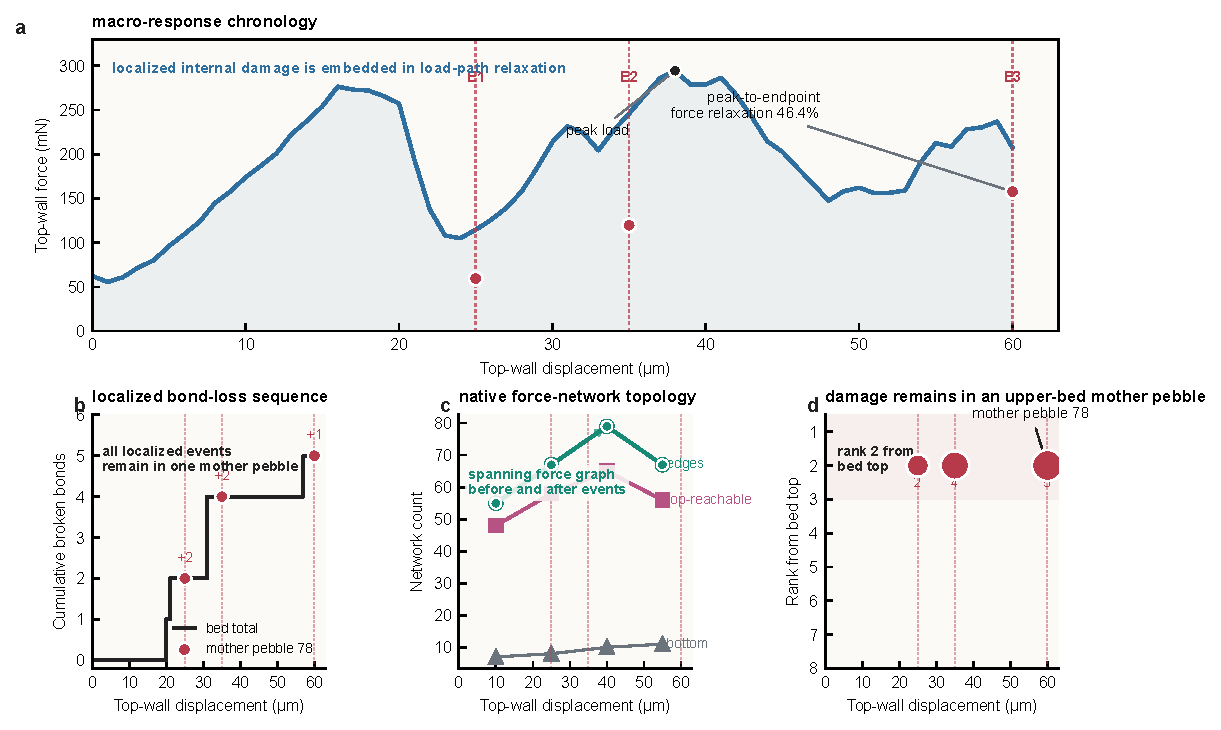
\includegraphics[width=0.92\textwidth]{pb007_corrected_fracture_sequence.pdf}
\caption{Corrected fracture-event sequence and native force-network evolution. a, Top-wall force and mother-pebble-resolved event windows during the 60 micrometre corrected compression pilot. b, Cumulative internal-bond loss from the thermo history with event-dump localization; all localized events occur in mother pebble 78. c, Native inter-mother force-network topology at sampled displacements, showing a spanning graph that densifies and then reorganizes. d, Height rank of damaged mother pebbles, identifying pebble 78 as a top-near but not geometrically highest mother pebble. Error bars are not shown because this is one corrected pilot sequence, not an ensemble statistic. The event-resolved representation complements earlier bulk crush-probability and crushable-bed approaches by revealing the time order and mother-pebble location of damage \cite{CrushProbabilityPebbleBed2011,Wang2021CrushableCeramicPebbleBed}.}
\label{fig:pb007-fracture-sequence}
\end{figure*}



\begin{table*}[!t]
\centering
\caption{Corrected fracture-sequence evidence.}
\label{tab:pb007-fracture-evidence}
\footnotesize
\resizebox{0.98\textwidth}{!}{%
\begin{tabular}{lllll}
\toprule
Quantity & Pilot bed & Intact independent bed and weakened-bond audits & Third independent bed & Interpretation \\
\midrule
Mother pebbles & 100 & 100 & 100 & Corrected 100-mother-pebble windows \\
Subparticles & 50,000 & 50,000 & 50,000 & 500 subparticles per mother pebble \\
Initial internal bonds & 493,500 & 493,500 & 493,500 & Bonded templates transferred intact \\
Final intact internal bonds at 60 micrometres & 493,495 & 493,500; 493,500 at 0.5x and 0.25x strength & 493,490 & Five lost bonds in the pilot; zero loss in the intact bed and strength audits; ten lost bonds in the third bed \\
Damaged mother pebbles & 1 & 0; 0 at 0.5x and 0.25x strength & 2 & Damage localizes in upper-bed mother pebbles \\
First thermo-resolved bond loss & 20 micrometres & none to 60 micrometres & 50 micrometres & Onset shifts with random local force-path topology \\
Event-dump increments & 25, 35 and 60 micrometres & none to 60 micrometres & 59 micrometres & Pilot: +2, +2 and +1 broken bonds; third bed: +10 across two mother pebbles \\
Final inter-mother force edges & 74 & 83; 83 in both strength audits & 63 & Native final contact-force topology \\
Final top-reachable mother pebbles & 57 & 67; 67 in both strength audits & 54 & Load-bearing graph remains spanning in all corrected cases \\
Final bottom-contacting mother pebbles reachable from top & 11 & 18; 18 in both strength audits & 7 & Native top-to-bottom force connectivity exists in all corrected cases \\
\bottomrule
\end{tabular}%
}
\end{table*}


Together, Fig. 5 and Table 1 support a localized, force-path-sensitive microcracking mechanism rather than bed-wide fragmentation within the simulated displacement range. In the corrected pilot, force-chain densification and reorganization precede the first event-localized internal bond loss, and subsequent microcrack growth remains confined to a single upper-bed mother pebble through 60 micrometres. The second independent corrected bed remains unbroken to the same displacement despite a spanning native force graph, including in the 0.5x and 0.25x strength-window audits. The third independent corrected bed adds a delayed-cracking path: it remains intact through the early and middle compression window, then loses ten bonds in two upper-bed mother pebbles after 50 micrometres while retaining a spanning native graph.


The corresponding macroscopic response shows why the event sequence should be interpreted as coupled bed restructuring rather than as an isolated single-bond trigger. In the pilot, the top-wall force reaches 0.294 N at 38 micrometres and then relaxes to 0.158 N at the 60 micrometre endpoint, after the event-localized bond losses at 25, 35 and 60 micrometres. The apparent secant response is therefore non-monotonic: it stiffens over the first two displacement windows and softens over the final 40-60 micrometre window. By contrast, the intact independent corrected bed reaches its peak force only at the 60 micrometre endpoint, 0.128 N, while retaining zero internal-bond loss. The delayed-cracking third bed reaches a higher endpoint force of 0.649 N, with the first bond loss at 50 micrometres and ten final broken bonds. The pilot and third bed also carry larger final inter-pebble force sums, 0.864 and 1.032 N, respectively, compared with 0.253 N in the intact independent bed, even though all corrected cases retain spanning native force graphs. A companion event-aligned topology table links the pilot bond-loss windows to the nearest native force-network states, showing that all three increments occur inside a measured spanning graph. These values are not treated as quasi-static elastic moduli; they are used as macroscopic signatures of contact-network reorganization, local load concentration and microcrack accommodation in small breeder-bed windows.


The same evidence can be organized as a compact set of material-degradation state variables (Table 2). This synthesis is useful for a nuclear-materials reader because it separates four levels that are often collapsed into a single breakage ratio: the internal damage chronology, the mother-pebble location of damage, the surrounding native force-network state and the macroscopic response of the bed window. The corrected pilot therefore does not merely report that five bonds failed; it reports when the failures occurred, where the damaged mother pebble sits in the packing, whether the load-bearing graph remained connected and how the force response changed while the internal event sequence unfolded. These state variables are the quantities that can later be passed to coupled thermal-contact, purge-flow or damage-accumulation models once larger ensembles become available.



\begin{table*}[!t]
\centering
\caption{Material-degradation state-variable synthesis from the corrected calculations.}
\label{tab:material-state-variables}
\footnotesize
\resizebox{0.98\textwidth}{!}{%
\begin{tabular}{llll}
\toprule
State variable & Evidence in corrected calculations & Materials interpretation & Current boundary \\
\midrule
Internal damage chronology & Pilot bond-loss increments of +2, +2 and +1 at 25, 35 and 60 micrometres; third bed first loses bonds at 50 micrometres and reaches +10 by the endpoint & Converts hidden pebble crushing into a time-ordered microcrack sequence & Three corrected 100-mother-pebble cases; not a fracture-probability distribution \\
Damaged mother-pebble identity & Pilot loss localizes in one rank-2 mother pebble; third-bed loss localizes in two rank-2/rank-3 mother pebbles & Identifies the local ceramic objects carrying early damage, rather than only a bed-average damage ratio & One independent corrected bed and strength audits remain intact to the same endpoint \\
Native force-network state & Pilot graph remains spanning with 74 endpoint inter-mother edges; intact bed has 83; delayed-cracking bed has 63 & Shows that local microcracking is embedded in a connected load-bearing skeleton & Force graph is reconstructed from sampled native local contacts \\
Macro-response accommodation & Pilot force relaxes from 0.294 N peak to 0.158 N at endpoint; intact bed peaks at 0.128 N; delayed-cracking bed reaches 0.649 N & Links microcracking and contact-network reorganization to bed-window stiffness evolution & Values describe finite 100-mother-pebble windows, not a bulk modulus \\
Negative strength-window audit & Independent bed stays intact at nominal, 0.5x and 0.25x bond strengths while retaining spanning topology & Rejects a deterministic displacement-only or strength-multiplier-only onset interpretation & Does not prove absence of fracture under other packings, rates or cyclic paths \\
Fusion-material relevance & Local damage coexists with force-chain densification, top-reachability growth and force relaxation & Provides state variables for future heat-transfer, purge-flow and damage-accumulation coupling & No coupled thermal-flow prediction is made here \\
\bottomrule
\end{tabular}%
}
\end{table*}


The corrected-case comparison in Fig. 6 makes this distinction explicit. The pilot carries higher top-wall loads over much of the early 60 micrometre window and develops three event-localized bond-loss increments. The second independent corrected bed retains zero internal-bond loss to the same endpoint under nominal, 0.5x and 0.25x bond-strength settings. The third independent corrected bed follows a delayed-cracking path, with no early damage but ten localized lost bonds after the force path has reorganized. All five calculations retain native force connectivity at the endpoint: the pilot finishes with 74 inter-mother edges and 11 bottom-contacting mother pebbles reachable from the top-loaded set, the intact independent-bed strength settings finish with 83 inter-mother edges and 18 bottom-contacting mother pebbles reachable from the top-loaded set, and the delayed-cracking bed finishes with 63 inter-mother edges and seven bottom-contacting mother pebbles reachable from the top-loaded set. The useful materials conclusion is therefore not that 60 micrometres always triggers fracture, or that a single bond-strength multiplier controls onset, but that the locked-template workflow can separate load-path formation from fracture onset and expose the local structural sensitivity of early breeder-pebble damage.


\begin{figure*}[!t]
\centering

\includegraphics[width=0.92\textwidth]{pb007_replicate_comparison.pdf}
\caption{Corrected-case comparison separates force connectivity from fracture onset. a, Top-wall force histories for the corrected pilot, the intact independent corrected bed, the delayed-cracking third corrected bed and the same intact bed with 0.5x and 0.25x bulk and weak-plane bond strengths. b, Event-localized cumulative internal-bond loss; pilot damage occurs in three mother-pebble event windows, the third corrected bed develops a delayed +10-bond event near the endpoint, and the intact bed plus weakened-bond audits remain unbroken to 60 micrometres. c, Native inter-mother force edges and top-reachable mother-pebble counts from pair/wall local dumps for the pilot, intact and delayed-cracking corrected beds; circles denote inter-mother edges and squares denote top-reachable mother pebbles. d, Endpoint mechanism fingerprint, showing each metric normalized to its own maximum across corrected cases and labelled for the pilot, intact and delayed-cracking beds. All corrected cases retain a spanning native force graph at the endpoint, but only two of the three independent bed geometries develop internal bond loss, indicating local force-path sensitivity rather than a deterministic displacement-only or bond-strength-multiplier threshold.}
\label{fig:pb007-replicate-comparison}
\end{figure*}


The result is therefore presented as event-sequence evidence from corrected 100-mother-pebble pilots, not as a converged fracture probability or a final design limit.


\section{Discussion}

This work demonstrates a corrected computational chain for resolving pebble-level fracture events inside random ceramic breeder beds in a fusion-blanket context. The key advance is not merely using a bonded particle model, but preserving each bonded template as an intact 1 mm mother pebble during bed formation, proving a native load-bearing contact graph before fracture, and then tracking its internal bond graph during compression. This sequence turns a conventional bed-compression calculation into a mesoscopic fracture diagnostic with explicit acceptance gates. Such diagnostics are directly relevant to blanket structural-integrity assessment because they identify where damage starts, whether it remains confined, and how the load-bearing topology changes around the first microcracking events. The event sequence therefore complements recent experiments that quantify bulk breakage ratio, fragment size and purge-gas pressure-drop consequences by supplying the otherwise hidden mother-pebble-resolved initiation history \cite{Fang2026Li4SiO4BedCrushing}.


The present evidence has three levels. First, at the single-pebble scale, the weak-plane template is a calibration candidate consistent with the available crush-load scale and split-type fragmentation morphology (Fig. 2). The controlled sensitivity set in Fig. 3 shows that first-break displacement and split topology are stable across 250-1000 subparticles and 0.03-0.10 m s$^{-1}$, although absolute peak load is not fully resolution- or rate-independent. Second, at the initialization scale, the surface-supported corrected route establishes a connected 100-mother-pebble bed and rejects protocols that either damage internal bonds during stiffness restoration or fail force-transmission checks (Fig. 4). Third, at the corrected fracture-sequence scale, the 60 micrometre pilot reveals a localized top-near microcracking sequence in one mother pebble while the native force network remains spanning and reorganizes (Fig. 5 and Table 1). A second independent corrected bed remains intact to 60 micrometres while retaining top-to-bottom native force connectivity, and remains intact in 0.5x and 0.25x strength-window audits of the same bed. A third independent corrected bed develops delayed upper-bed microcracking after 50 micrometres and ends with ten broken bonds in two mother pebbles while still retaining a spanning native force graph. These results suggest that early breeder-bed degradation may begin as localized upper-bed microcracking embedded in a changing force network, but they also show that the onset is strongly controlled by local random packing and force-path topology.


From a nuclear-materials perspective, this event order matters because the first mechanically degraded pebble is not simply a lost strength point in an otherwise unchanged packing. In the corrected pilot, the damaged mother pebble remains part of a spanning native contact graph while the inter-mother edge count, top-reachable population and macroscopic force response reorganize around it. A post-processing mechanism audit quantifies this contrast: the endpoint broken-bond fraction is only 1.0e-5, but the inter-mother edge count densifies by 1.44x before reorganization, the top-reachable population by 1.35x, and the peak-to-endpoint top-wall force relaxes by 46.4\%. The simulated microcrack sequence therefore identifies a local defect that can change contact stiffness and contact area before producing bed-wide fragmentation. In a blanket, the same class of localized contact-network rearrangement would be expected to perturb heat-transfer constrictions and helium purge-flow tortuosity near the damaged region, even when the global bed still appears mechanically connected. The present model does not yet solve coupled thermal or flow transport, but it supplies the missing fracture-event chronology and native force-network state variables that such coupled degradation models require. This is the materials value of the event-sequence formulation: it converts a small number of internal bond failures into a time-stamped, location-resolved and load-path-aware description of ceramic breeder-bed degradation.


The topology descriptors also give the calculation a damage-mechanics interpretation. The first broken bonds are not triggered in an isolated pebble with a fixed external load; they occur in a mother pebble that is embedded in a changing contact skeleton. The measured increase and subsequent reorganization of inter-mother force edges indicate that the bed can both concentrate load into a vulnerable local region and redistribute load after a small amount of internal damage. In this sense, the force network acts as a mesoscale shielding-and-activation field for ceramic microcrack initiation. Reporting the event time, mother-pebble identity, height rank, native reachability and macroscopic force relaxation together is therefore more informative for breeder-material degradation than reporting a final broken-bond count alone.


This conclusion is intentionally narrower than the interpretation suggested by the early diagnostic calculations. Those superseded calculations remain useful as a methodological caution: zero internal-bond loss after template insertion is not by itself enough to claim a valid bed-scale fracture sequence if native force transmission is absent or poorly validated. For a Journal of Nuclear Materials audience, this is a materials-modelling point rather than a software point: the integrity of the simulated ceramic microcrack sequence depends on proving that the parent pebble experiences a physically meaningful bed contact environment before bond loss is interpreted. The corrected route therefore shifts the manuscript from a large but insufficiently validated event database to a smaller, acceptance-gated fracture sequence with native force-network evidence.


Several limitations define the next stage before the method can support quantitative blanket design. The single-pebble template is a current calibration candidate, not a final Li$_4$SiO$_4$ material law; experimental elastic-stiffness calibration and larger stochastic strength ensembles are still needed. The three 60 micrometre corrected beds and the 0.5x/0.25x strength audits provide event-sequence and sensitivity evidence, not a converged failure probability. Robust design-margin estimates will require additional independent corrected beds, orientation ensembles, lower-rate or hold-relaxation loading, cyclic and temperature-dependent paths, and coupling to thermal contact conductance and purge-flow metrics. Within these limits, the present workflow provides a defensible route for converting bonded-particle bed simulations into auditable fracture-event sequences for ceramic breeder-material assessment, with no coupled thermal-flow prediction made in the present study.


\section{Conclusions}

This study establishes an acceptance-gated bonded-template route for resolving early fracture events in Li$_4$SiO$_4$ ceramic breeder beds. The main contribution is methodological and mechanistic: intact 500-subparticle mother-pebble templates are inserted into random beds without seating damage, invalid load-path cases are rejected by native force-connectivity and force-balance gates, and subsequent compression is converted into mother-pebble-resolved bond-loss and force-network histories. The corrected evidence shows that early damage can remain highly localized in upper-bed pebbles while the bed-scale force graph remains spanning and reorganizes: one bed develops five localized broken bonds, a second remains intact even under weakened-bond audits, and a third develops delayed ten-bond microcracking after 50 micrometres. The resulting workflow provides a reproducible computational diagnostic for ceramic breeder-material degradation, while quantitative blanket design margins require larger stochastic ensembles and additional thermomechanical coupling.


\section{Methods Summary}

Simulations used a local no-VTK LIGGGHTS-INL 4.0.0 build \cite{LIGGGHTSINL} with SI units, granular atoms and a Hertzian tangential-history cohesive-bond contact law with stress-based bond breakage and disabled automatic bond creation after initialization. Unless otherwise noted, bonded-template calculations used a 5.0 ns timestep, density 2400 kg m-3, Young's modulus 90 GPa, Poisson ratio 0.25, restitution coefficient 0.3 and friction coefficient 0.5. The selected weak-plane template used 500 subparticles, bond stiffnesses of 1.0e14 and 5.0e13 N m-3, bulk normal and tangential strengths of 90 MPa in the bed runs, weak-plane strengths of 22.5 MPa, a 0.20 mm bulk bond-creation distance and a 0.09 mm weak-plane creation distance. Single-pebble calibration runs used the same contact formulation, with parameter scans around this weak-plane family retained only as calibration evidence.


For the subparticle-count sensitivity study, 250-, 500- and 1000-subparticle templates were generated with the same random seed, 0.30 nominal internal solid fraction and a minimum centre spacing of 2.05 subparticle radii. The 500-subparticle geometry exactly reproduced the archived reference template. Bulk and weak-plane bond-creation distances were scaled with subparticle radius from the 500-subparticle values of 0.20 and 0.09 mm, while bond stiffnesses and strengths were held fixed. All three templates were compressed to 0.30 mm at 0.10 m s$^{-1}$ using the same plate-generation protocol. The matched-rate study used the 500-subparticle template and identical boundaries at 0.10, 0.05 and 0.03 m s$^{-1}$; step counts were adjusted so that every run reached the same 0.30 mm endpoint.


Table 3 summarizes the material, contact and bonded-template parameters used in the accepted single-pebble and corrected-bed calculations.



\begin{strip}
\vspace{-0.6\baselineskip}
\centering
\captionof{table}{Model and bonded-template parameters used in the present simulations.}
\label{tab:model-parameters}
\scriptsize
\resizebox{0.98\textwidth}{!}{%
\begin{tabular}{llll}
\toprule
Parameter & Value & Used in & Notes \\
\midrule
Mother-pebble nominal diameter & 1.0 mm & Single pebble and beds & Representative Li$_4$SiO$_4$ breeder pebble size used for all mother pebbles \\
Subparticles per mother pebble & 500 & Bonded template & Random non-overlapping subparticle template \\
Initial internal bonds per inserted template & 4935 & Corrected bed insertion and compression & Required before accepting a corrected bed compression run \\
Particle density & 2400 kg m-3 & Contacts and template mass & Representative Li$_4$SiO$_4$ density \\
Young's modulus & 90 GPa & Hertzian contacts & Used with Poisson ratio 0.25 \\
Poisson ratio & 0.25 & Hertzian contacts & Same value used in single-pebble and bed runs \\
Restitution coefficient & 0.3 & Contacts & Numerical damping through the contact law \\
Friction coefficient & 0.5 & Contacts & Particle-particle and particle-wall contacts unless otherwise stated \\
Bond normal stiffness & 1.0e14 N m-3 & Cohesive bonds & Selected after stiffness screening; higher stiffness was excluded pending smaller-timestep checks \\
Bond tangential stiffness & 5.0e13 N m-3 & Cohesive bonds & Set to half of the normal stiffness \\
Bulk bond normal/tangential strength & 90 MPa & Selected weak-plane template in bed runs & Same nominal strength used for bonds away from the weak plane \\
Weak-plane bond normal/tangential strength & 22.5 MPa & Selected weak-plane template & One quarter of the bulk strength \\
Bulk bond-creation distance & 0.20 mm & Template generation & Forms the main internal bond network \\
Weak-plane bond-creation distance & 0.09 mm & Template generation & Reduces cross-plane connectivity and promotes split-type fracture \\
Selected weak-plane orientation & x-normal & Reference single-pebble and bed template & Other orientations were used only as sensitivity checks \\
Single-pebble loading velocities & 0.10, 0.05 and 0.03 m s$^{-1}$ & Matched-boundary rate sensitivity & All three runs reach 0.30 mm displacement \\
Step-relaxed displacement increment & 1 micrometre & Corrected bed validation and fracture pilot & Each increment is followed by relaxation before the next loading step \\
Bonded-template timestep & 5.0 ns & Single-pebble and bed compression & Checked with granular timestep monitor \\
Proxy-settling timestep & 1.0 us & Gravity deposition & Used only for unbonded proxy-sphere settling \\
Corrected pilot bed size & 100 mother pebbles & Corrected validation and fracture sequence & Used for the current acceptance-gated event-sequence evidence \\
\bottomrule
\end{tabular}%
}
\vspace{-0.6\baselineskip}
\end{strip}


Random beds were generated in two stages. First, 1.0 mm proxy spheres were inserted into an 11 mm by 11 mm lateral box and settled under gravity using an unbonded Hertzian contact law, a 1.0 us timestep and viscous damping until the tail kinetic energy was small. Second, the settled proxy centres were replaced by bonded 500-subparticle templates. Templates were initially created far apart so that bonds formed only within each mother pebble; the atom-id groups were then translated to the proxy centres. For the corrected route, the initialization check required the exact expected bond count, 4935 internal bonds per mother pebble and 493,500 bonds for the 100-mother-pebble bed, before any compression step was accepted.


The corrected bed used rigid-clump settling followed by bonded-template transfer. For the 100-mother-pebble pilot, the bonded transfer produced 50,000 subparticles and 493,500 initial internal bonds. The pre-damage validation stage used step-relaxed top-wall loading with five 1 micrometre increments. The bottom wall already supports self-weight after settling, so force transmission was assessed by subtracting the last zero-top-force gravity baseline and comparing the top-wall load with the incremental total six-wall vertical force.


The corrected fracture pilot used the same acceptance-gated entry protocol with restored contact modulus 1.5e10 Pa, 10,000 pre-compression relaxation steps and 1 micrometre step-relaxation increments continued to 60 micrometres. The independent-bed strength-window audits used the same corrected bed and compression endpoint, but reduced bulk normal/tangential strengths from 90 MPa to 45 and 22.5 MPa, and weak-plane normal/tangential strengths from 22.5 MPa to 11.25 and 5.625 MPa. A third independent random bed was generated with a separate insertion seed, passed the same 600,000-step rigid-settling and 5 micrometre loaded-endpoint entrance gates, and was then compressed to 60 micrometres under the same no-hold protocol. Periodic local internal-bond dumps were written during compression, together with native pair and wall local dumps. Bond status was recorded with \texttt{compute bond/counter}; intact internal bond pairs were written using \texttt{compute pair/gran/local/bond} and \texttt{dump local}. Mother-pebble events were obtained by comparing each local dump with the reference intact internal bond graph, assigning atom-id ranges to mother-pebble ids, and counting positive increments in broken internal bonds as localized events. Native inter-mother force-network metrics were reconstructed directly from the pair and wall local dumps, not from overlap proxies. Top-wall force histories, peak-force locations, endpoint forces and displacement-window secant slopes were extracted from the thermo output. The inter-pebble force sum was computed by aggregating the magnitudes of native local contact forces between distinct mother-pebble ids at the sampled endpoint. These macroscopic and graph metrics were used to compare response evolution among corrected cases, not to report a bulk elastic modulus for the finite 100-mother-pebble window.


\section{Data availability statement}

The processed event tables, native force-network summaries, event-aligned topology table, macro-topology-event metrics, figure source data, manuscript figures and post-processing scripts supporting this study have been assembled in a reduced reproducibility package with a checksum manifest. The package includes the corrected pilot, the intact independent corrected bed, the delayed-cracking third corrected bed and the 0.5x/0.25x strength-audit thermo histories, mother-pebble bond-series tables, breakage-event tables, native force-network series, Fig. 6 source data and the scripts used to regenerate the replicate-comparison figure, event-aligned topology table and mechanism-metric table. The package has been deposited in a persistent repository and is available at https://doi.org/10.5281/zenodo.20687351. Very large raw restart files and full local-bond dump histories are retained as local case archives and can be provided as larger audit bundles on reasonable request, subject to repository file-size limits and institutional storage constraints.


\section{Code availability statement}

The template-generation, run-control, figure-generation and post-processing scripts are included in the reduced reproducibility package under \texttt{scripts/}, with representative DEM input files under \texttt{simulations/}. The deposited package is intended to reproduce the manuscript-level processed data audits, figures and evidence matrices from the included CSV tables and representative inputs; it does not redistribute the local DEM executable, very large restart files or full raw local-bond dump histories. The simulation environment used for the reported calculations is stated in the Methods Summary, and the package manifest provides SHA256 checksums for the deposited scripts, inputs, processed data and figures.


\section{Acknowledgements}

This work was supported by the Anhui Provincial Natural Science Foundation (2408085QA030), the Science Foundation of the Institute of Plasma Physics, Chinese Academy of Sciences (DSJJ-2025-08), the Anhui Intelligent Mine Technology and Equipment Engineering Research Center (AIMTEERC202307), the China Post-doctoral Science Foundation under Grant Number 2024M753266, the Excellent Research and Innovation Team of Anhui Province, China (2022AH010052), the Scientific Research Foundation for High-level Talents of Anhui University of Science and Technology, China (2021yjrc51), and the Collaborative Innovation Program of Hefei Science Center, CAS, China (2019HSC-CIP006).


\section{Role of the funding source}

The funding sources had no role in the design of the computational study, the collection, analysis or interpretation of the simulation data, the writing of the manuscript, or the decision to submit the article for publication.


\section{Author contributions}

Jian Wang: Validation, Supervision, Project administration, Methodology, Investigation, Conceptualization. Siyu Wang: Writing - original draft, Formal analysis, Data curation, Visualization. Hang Zhang: Writing - original draft, Formal analysis, Data curation, Visualization. Ming-Zhun Lei: Writing - review and editing, Validation, Project administration, Formal analysis. Wei Wen: Writing - review and editing, Supervision, Project administration, Methodology, Conceptualization. Qi-Gang Wu: Validation, Resources, Data curation. Gang Shen: Writing - review and editing, Supervision, Project administration. Haishun Deng: Supervision, Project administration.


\section{Declaration of generative AI and AI-assisted technologies in the writing process}

During the preparation of this work, the authors used OpenAI's ChatGPT/Codex tools to assist with manuscript organization, language editing, code review, figure-generation scripting and submission-package preparation. After using these tools, the authors reviewed, edited and verified the manuscript text, code, figures and data products as needed, and take full responsibility for the content of the publication.


\section{Declaration of competing interest}

The authors declare that they have no known competing financial interests or personal relationships that could have appeared to influence the work reported in this paper.



\bibliographystyle{elsarticle-num}
\bibliography{references}
\end{document}
